% copyrights (c) Hamza Ba-mohammed - ENSIAS UM5 Rabat Morocco
% Artificial Intelligence Branch - season 2022/2023
\documentclass{beamer}
\usepackage[english]{babel}
\usepackage{amsfonts}
\usepackage{amsmath}
\usepackage{amssymb}
\usepackage{graphics}
\usepackage{array}
\usepackage{xcolor}
\usepackage{setspace}
\usepackage{wrapfig}

% add more libraries here if you need them
\usepackage[font=scriptsize]{caption}
\usepackage{hyperref}

\title[Turbomachinary]{Simple $H_2O_2$ monopropellant rocket engine}

\author[Khue Q. Tran]{Presented by:\\
\textbf{Khue Q. Tran}\\
% In front of the jury:\\
% \textbf{Mr. jury 1} and
% \textbf{Mr. jury 2}\\
% Supervised by:\\
% \textbf{Mr. supervisor 1} (Internal)\\
% \textbf{Mr. supervisor 01} and \textbf{Mr. supervisor 02} (External)
}

\date{January $5^{th}$ 2023}

%\logo{
%\includegraphics[width=1cm]{images/ensias.png} % school logo
%\includegraphics[width=1cm]{images/ensias.png} % company logo
%}

\usetheme{CambridgeUS} % you can change it on choice
% I recommend: CambridgeUS, Berlin, Singapore
% for more choices, visit: https://deic.uab.cat/~iblanes/beamer_gallery/index_by_theme_and_color.html



\begin{document}
{
\usebackgroundtemplate{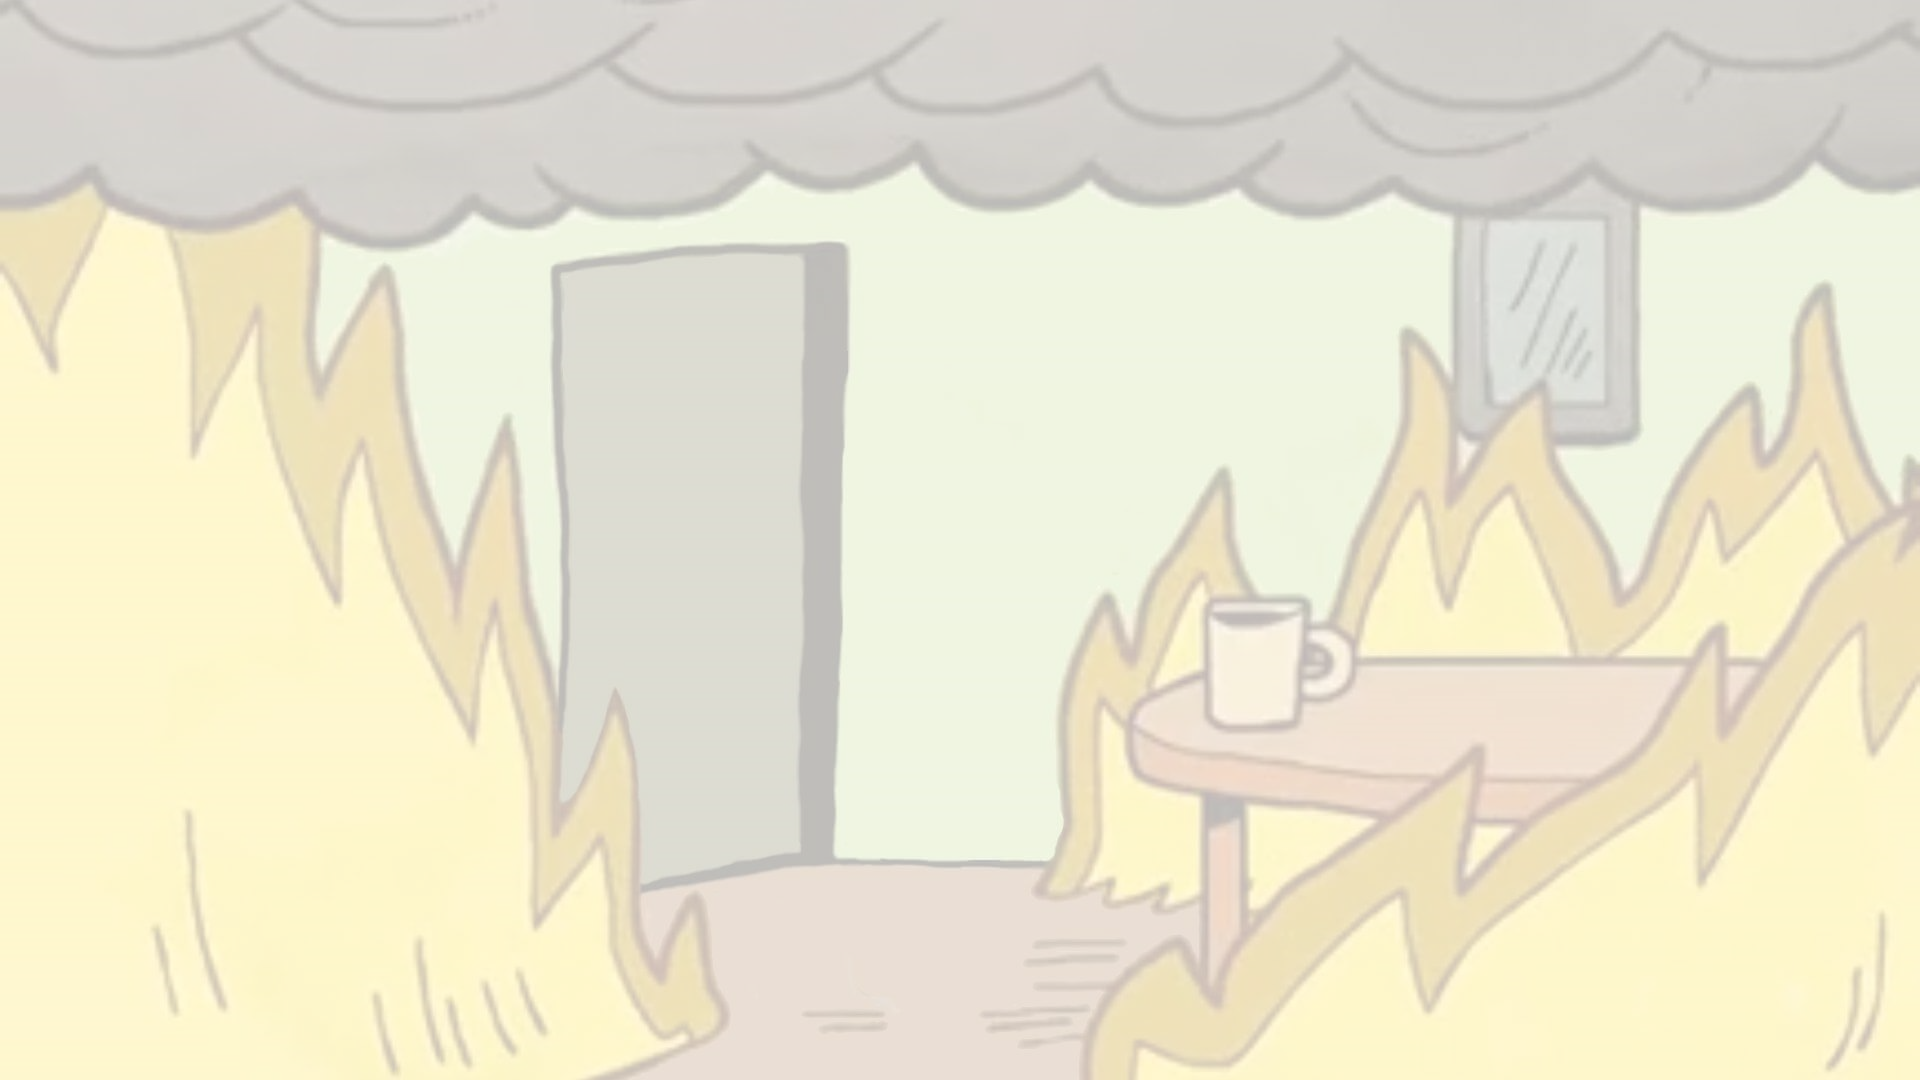
\includegraphics[width=18cm]{images/bg.png}}% make sure to reduce the opacity of the BG before uploading it
\begin{frame} 
    \maketitle
\end{frame}
}

\section*{Table of conents}
\begin{frame}
    \tableofcontents
\end{frame}

\addtocontents{toc}{\setcounter{tocdepth}{2}} % to show more deep subparts, increment the number "1" to 2 or 3...


% generally, this is the structure of a thesis defense. you can keep it
%=======================================================================================
\section{Introduction}

\subsection{Safety}
\begin{frame}{Safety}
    A rocket engine is always dangerous due to the release of gas and energy! 
    For this rocket engine design, the propellant is high concentration of hydrogen peroxide  ($H_2O_2$). 
    \begin{itemize}
        \item At low concentration, $H_2O_2$ is safe and used widely for household applications. However, at high concentrations, $H_2O_2$ is dangerous due to its oxidizing properties that could lead to skin burn in contact.
        \item $H_2O_2$ is not stable, may decompose into oxygen and water, and release a lot of energy. This decomposition happens rapidly and lead to damages
        \item $H_2O_2$ is not compatible with commons materials: brass (usually used for pneumatics equipments), buna rubber (usually in O-rings/sealing), oil-based grease. The construction materials should be stainless steel or aluminum, Teflon-based O-rings/sealing and grease.
    \end{itemize}
\end{frame}

%----------------------------------------------------------------------------------------
\subsection{System requirements}

\begin{frame}{Mission type}
    \begin{columns}
        \begin{column}{0.6\textwidth}
        \noindent
        The concept mission is a small lander:
        \begin{itemize}
            \item Thrust adequate for the lander: $250N$
            \item Required burn time: $40s$
            \item Ease to ignite and shut down
            \item Low cost and ease to manufacture
        \end{itemize}
        \end{column}
    
        \begin{column}{0.4\textwidth}
        \begin{figure}[t]
            \centering
            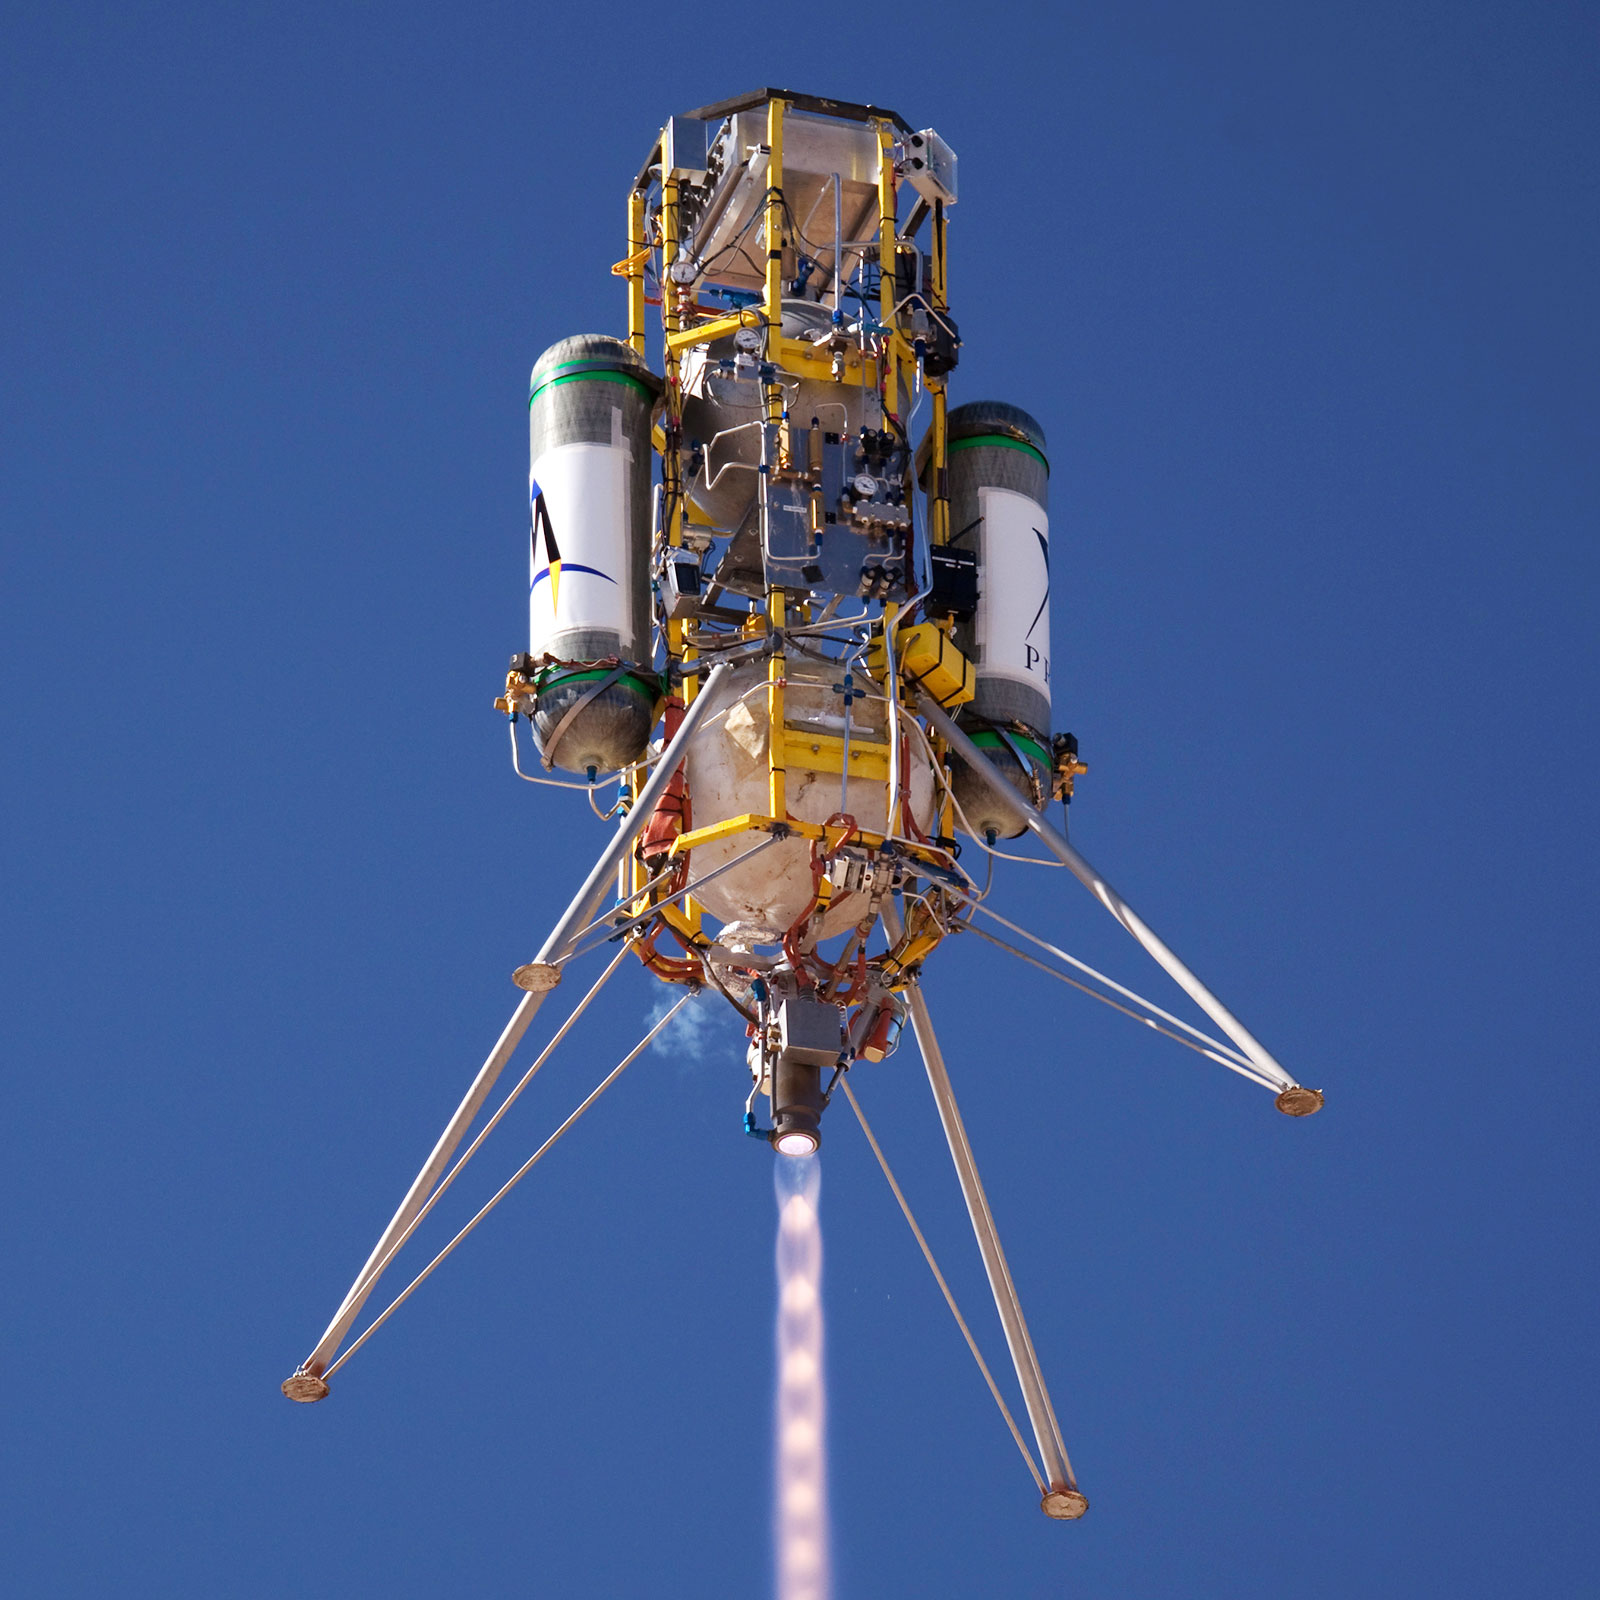
\includegraphics[width=0.9\linewidth]{images/masten-xombie-square.jpg} 
            \caption{Masten Xombie test vehicle}
        \end{figure}
        \end{column}
    \end{columns}
\end{frame}

%=======================================================================================
\section{Rocket engine principle}

%----------------------------------------------------------------------------------------
\subsection{de Laval nozzle}
\begin{frame}[t]{de Laval nozzle}
    \noindent
    \begin{minipage}[t]{0.55\textwidth}
        \vspace{-10pt}
        \begin{itemize}
            \item At the convergence section, the flow is "choked" to sonic flow. Theoretically, any further reduction in cross-section does \textbf{not} increase the flow velocity. Theoretically, the ratio between divergence section inlet and the throat is about $1.5$. 
            \item At the divergence section, the flow is accelerated to supersonic flow. The divergence section expansion ratio depends on the ratio between inlet and ambient pressure. In case of vacuum, the limit factor of expansion ratio is surface tension and condensation of the fluid.
        \end{itemize}
    \end{minipage}%
    \hfill
    \begin{minipage}[t]{0.45\textwidth}
        \vspace{-5pt}
        \begin{figure}[t]
            \centering
            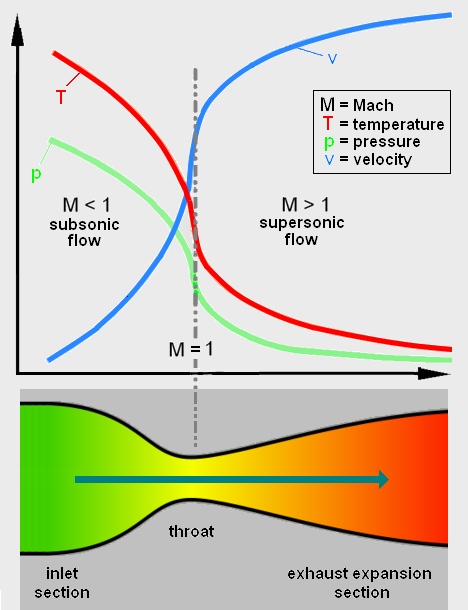
\includegraphics[height=0.65\textheight]{images/De_Laval_nozzle.png}
        \end{figure}
    \end{minipage}
    
\end{frame}

\begin{frame}
    The values usually use to parameterize the nozzle's geometry
    \begin{itemize}
        \item Throat diameter: from characteristics thrust CF
    \end{itemize}
    Divergence section
    \begin{itemize}
        \item Exit diameter: from expansion ratio $A_t / A_e$
        \item Divergence half angle $\alpha$, usually $15^{\circ}$
    \end{itemize}
    Convergence section
    \begin{itemize}
        \item Combustion chamber length: based on combustion, O/F mixing...
        \item Combustion chamber diameter: from conctraction ratio
        \item Convergence half angle $\theta$, usually in the range of $20^{\circ}$ to $45^{\circ}$
    \end{itemize}
    \centering  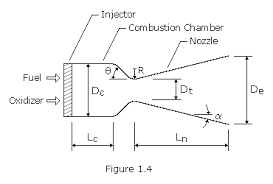
\includegraphics[height=0.45\textheight]{images/combustion_chamber_parameters.png}
\end{frame}

\begin{frame}[t]{Design parameter for a de Laval nozzle}
    \noindent
    \begin{minipage}[t]{0.6\textwidth}
        \vspace{-5pt}
        \begin{itemize}
            \item Throat size $\rightarrow$ Depends on mass flow rate through the nozzle
            \item Throat expansion ratio, which affects divergence section length is $A_{exit}/A_{inlet}$ $\rightarrow$ Depends on pressure ratio between combustion chamber and ambient, and combustion enthalpy
            % \item Combustion chamber length, combustion chamber diameter and convergence section length length are usually from real testing
            \item Convergence and divergence half angles are calculated from real fluid's surface tension, boundary layer, Raynold number
            $\rightarrow$ For an ideal nozzle without any loss, the nozzle could be an orifice. In practice, these angles are usually in a consistent range
        \end{itemize}
    \end{minipage}%
    \hfill
    \begin{minipage}[t]{0.35\textwidth}
        \vspace{30pt}
        \begin{figure}[t]
            \centering
            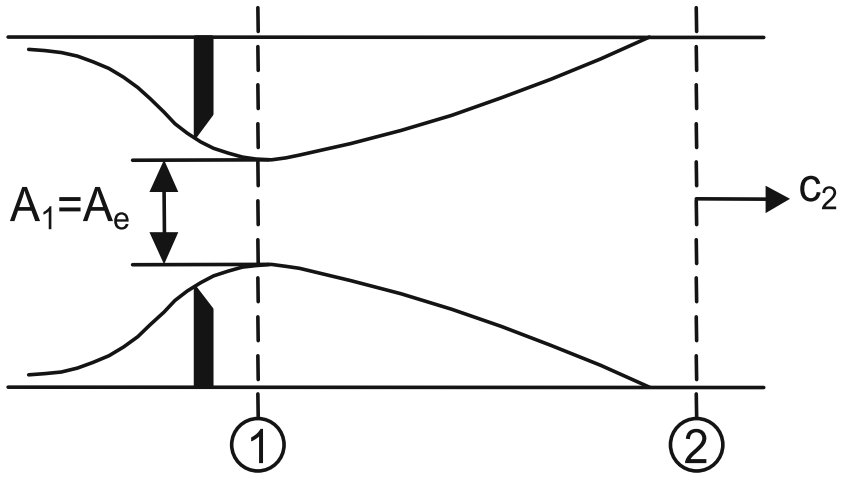
\includegraphics[width=\textwidth]{images/orifice_nozzle.png}
        \end{figure}
    \end{minipage}    
\end{frame}

\begin{frame}[t]{Design parameter for a de Laval nozzle}
    \begin{itemize}
        \item Combustion chamber length depends on the combustion, fuel-oxidizer mixing... and usually no trivially numerical results, results are mostly from testing.
        \item Combustion chamber diameter depends on contraction ratio between $A_{chamber} / A_{throat}$. Ideally, this ratio is about 1.5, but due to boundary layer, turbulent flow... this value is larger than ideal value
        \item Convergence half angle $\Theta$ is usually in the range of $20^{\circ}$ to $45^{\circ}$
    \end{itemize}
    \centering 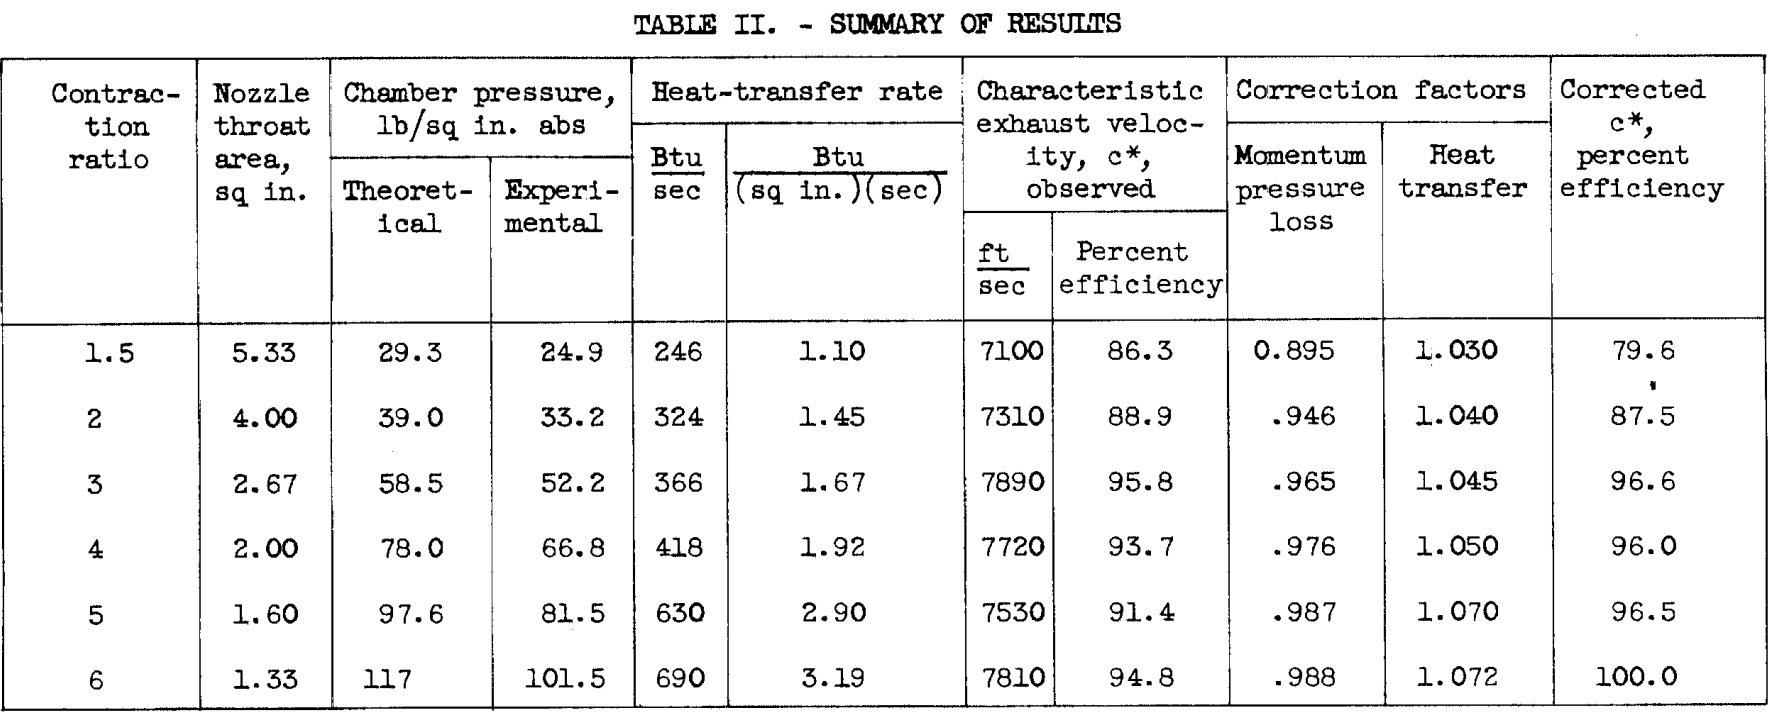
\includegraphics[height = 0.5\textheight]{images/combustion_contraction_ratio.png}
\end{frame}

%----------------------------------------------------------------------------------------
\subsection{Pressure-fed cycle}
\begin{frame}{Pressure-fed cycle}
    \begin{figure}[t]
        \centering
        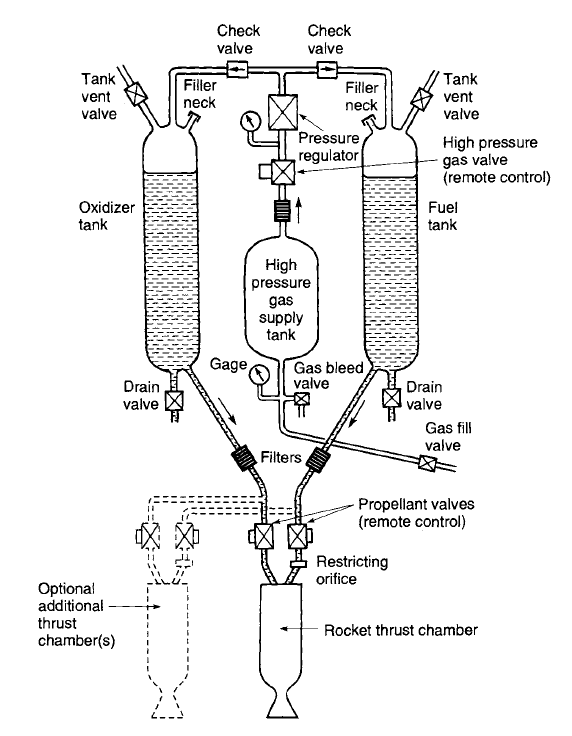
\includegraphics[height=0.84\textheight]{images/pressure_fed_cycle.png}    
    \end{figure}
\end{frame}

%----------------------------------------------------------------------------------------
\subsection{Hydrogen peroxide}

\begin{frame}{Why Hydrogen peroxide?}
    \begin{itemize}
        \item Hydrogen peroxide is a liquid at room temperature and pressure \\ $\rightarrow$ Could be easily stored and require no thermal insulation
        \item Could decompose and release energy without the presence of other fuels 
        \\ $\rightarrow$ Does not require complex system compared with bipropellant
        \item The decomposition is autogenous with catalyst 
        \\$\rightarrow$ Ease to ignite and restart
        \item Safe (with low concentration) 
        \\$\rightarrow$ In case of malfunction, hydrogen peroxide could be easily neutralized by diluting with water
    \end{itemize}
\end{frame}

\begin{frame}{Hydrogen peroxide decomposition}
    The decomposition of $H_2O_2$ \\
    \begin{center}
        $2H_2O_2 \rightarrow 2 H_2O + O2$ \        
    \end{center} 
    generates $\Delta H = –2884.5 kJ/kg$ at standard condition $T=25^{\circ}C, 1\:atm$ \\

    This decomposition usually requires a catalyst. Usually, the catalyst used is silver (both in pure form or silver coated) \\

    \begin{figure}
        \centering
        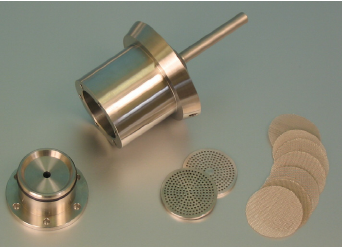
\includegraphics[height=0.35\textheight]{images/Catalyst-bed-composition.png}
        \caption{Silver mesh catalyst bed}
    \end{figure}
\end{frame}


%=======================================================================================
\section{Development}

%----------------------------------------------------------------------------------------
\subsection{Engineering consideration}

\begin{frame}{Engineering consideration}
    \begin{itemize}
        \item The engine runs on a pressure-fed cycle
        \item High-pressure gas supply tank is limited to 300 bar (30MPa)
        \item The engine runs by $H_2O_2$ monopropellant (the energy is from the decomposition of $H_2O_2$ only)
        \item The concentration of $H_2O_2$ is 80\%
    \end{itemize}
\end{frame}

%----------------------------------------------------------------------------------------
\subsection{Sample chamber-nozzle geometry calculation}
\begin{frame}{First law of thermodynamics}
    Rocket engine is the heat engine, which must satisfy the first law of Thermodynamics for flow in an adiabatic nozzle \\
    \begin{center}
        $h_2 - h_1 = -\frac{1}{2}\times(c_2^2 - c_1^2)$
    \end{center}    
    For non-ideal gas, the enthalpy is the function of $H(pressure, Temperature)$. There are no such models universally, to determine these enthalpy values \\
    $\rightarrow$ The enthalpy values usually come from real measurement, and complex state equations, for each kind of substance! Usually, we use numerical software to calculate the thermodynamic properties of the rocket engine.
\end{frame}

\begin{frame}{NASA CEA demo for thermodynamics calculation}
    Initial conditions
    \begin{itemize}
        \item $H_2O_2$ 80\% monopropellant (20\% left is water)
        \item Combustion chamber pressure is 30 bar, ambient pressure is 1 bar, ratio=30
        \item Initial $H_2O_2$ temperature: 293.15K
    \end{itemize}
    \vspace{10pt}
    \centering \url{https://cearun.grc.nasa.gov/}
\end{frame}

\begin{frame}{Sample NASA CEA result}
    \centering 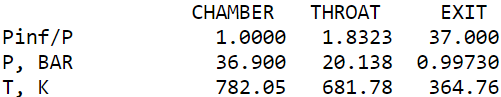
\includegraphics[width=0.6\textwidth]{images/combustion_temperature_example_cea.png} \\
    \vspace{15pt}
    \centering 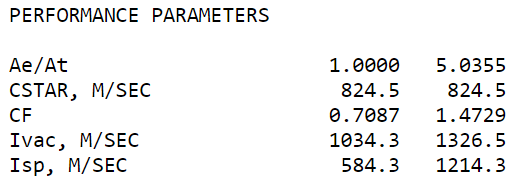
\includegraphics[width=0.6\textwidth]{images/example_cea_perf_params.png} \\
\end{frame}

\begin{frame}{Sample chamber-nozzle geometry calculation}
\begin{itemize}
    \setlength\itemsep{0.5em}
    \item The combustion temperature is 782.05K ($508.9^{\circ}C$. It is a relatively low value for metal materials. Hence, it does not require to cool down the engine, and no need to calculate heat transfer
    \item For the required thrust of 250N, the required mass flow rate is
    \begin{center}
        $\dot{m}[kg] = \frac{F_{thrust}[N]}{Isp[m/s]} = \frac{250N}{1214.3m/s} = 0.206kg/s$ 
    \end{center}
    \item Throat area
    \begin{center}
        $A_t[in^2] = \frac{F_{thrust}[lbf]}{C_f \times p_{chamber}[psi]} = \frac{56.2lbf}{1.4729 \times 435.1psi} = 0.0877in^2 = 56.59mm^2$
    \end{center} \\
    $\rightarrow$ The throat diameter $D_{throat}$ = 8.5mm
    \item Nozzle exit diameter
    \begin{center}
        $D_{exit} = D_{throat} \times \sqrt{\frac{A_{exit}}{A_{throat}}} = 8.5mm \times \sqrt{5.0355} = 19.1mm$
    \end{center}
\end{itemize}
\end{frame}

\begin{frame}{Sample chamber-nozzle geometry calculation}
    For this simple engine, some characteristics properties are
    \begin{itemize}
        \item Geometry is linear (which is about 93\% efficiency)
        \item Combustion chamber-throat concentration: 2.5 \\
        $d_{chamber} = d_{throat} \times \sqrt{{contraction\:ratio}} = 8.5mm \times \sqrt{2.5} = 13.44mm$
        \item Combustion chamber length/diameter ratio: 4
        $L_{chamber} = d_{chamber} \times \frac{L}{D} = 13.44mm \times 4 = 53.76mm$
        \item Converging half angle: $\Theta = 30^{\circ}$
        \item Diverging half angle: $\alpha = 15^{\circ}$
    \end{itemize}
\end{frame}

\begin{frame}{Sample chamber-nozzle geometry calculation}
    \centering 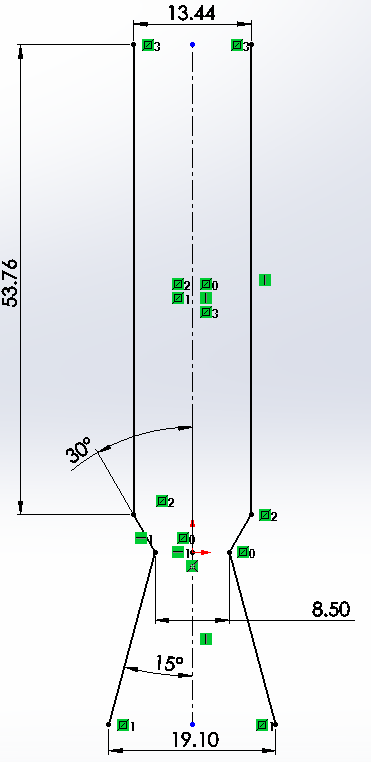
\includegraphics[height = 0.85\textheight]{images/sample_chamber_nozzle_geometry.png}
\end{frame}

%----------------------------------------------------------------------------------------
\subsection{Sample chamber-nozzle thickness calculation}
\begin{frame}{Sample chamber-nozzle thickness calculation}
    Due to manufacturing constraints, the nozzle assembly is 3D-printed, AlSi10Mg alloy. This material has tensile strength of 210MPa. Safety factor for this engine is at least $SF=2$ . There are 3 consumptions 
    \begin{itemize}
        \item The material loss 30\% percent of its strength at 782.05K
        \item The thickness is the same for the whole assembly. The 3D-printed part strength is homogeneous in all directions
        \item The stress is highest at combustion chamber
    \end{itemize}
    Hoop (Circumferential) Stress for thin-walled vessel
    \begin{center}
        $\sigma_h \times SF = \frac{pd}{2t}$
    \end{center}
    Longitudinal (Axial) Stress for thin-walled vessel \\
    \begin{center}
        $\sigma_l \times SF = \frac{pd}{4t}$
    \end{center}
    $\Rightarrow{t = 2.5mm}$ with SF = 2.3
\end{frame}

\begin{frame}
    \centering 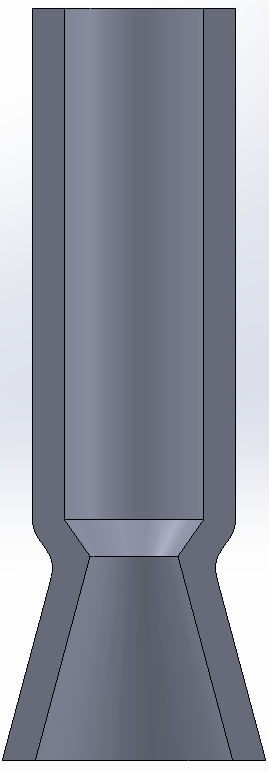
\includegraphics[height=0.9\textheight]{images/chamber_nozzle.png}
\end{frame}


%----------------------------------------------------------------------------------------
\subsection{Simple injector}

\begin{frame}{Simple injector}
A rocket engine injectors has two main contributions
    \begin{itemize}
        \item Mix the fuel and oxidizer
        \item Act as a flow-restricting orifice to prevent the combustion gas to blow-back into feed line. This is different from normal injector that used in internal-combustion engine as rocket engine is a continuously flow engine
    \end{itemize}
\centering 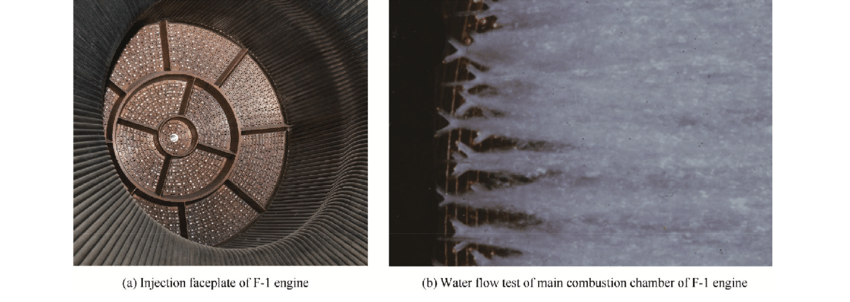
\includegraphics[height=0.5\textheight]{images/saturn_v_f1_injector.png}
\end{frame}

\begin{frame}
    \begin{itemize}
    \item For our simple $H_2O_2$ engine, there is no mixing as our engine is monopropellant. \\
    $\rightarrow$ The nozzle could be a simple spray nozzle. \\
    \item For combustion stability, the pressure drop through the injector is 15\% to 20\% \\
    $\rightarrow$ For combustion pressure of 30 bar, the pressure drop is 6 bar.
    \item Also, as the mass flow rate is $\dot{m} = 0.206kg/s$ and $\rho_{H_2O_2} = 1.4kg/l$, the volumetric flow rate is $\dot{V} = 0.2884$l/s $= 4.57gpm$ (gallon per minute)\\
    \end{itemize}

    \noindent
    \begin{minipage}[t]{0.65\textwidth}
        From volumetric flow rate and pressure drop, we could find the spray nozzle orifice diameter (ISO 5167 standard for spray nozzle). An online tool: \url{http://www.pressure-drop.com/Online-Calculator/index.html}
    \end{minipage}%
    \hfill
    \begin{minipage}[t]{0.35\textwidth}
        \vspace{-5pt}
        \begin{figure}[t]
            \centering 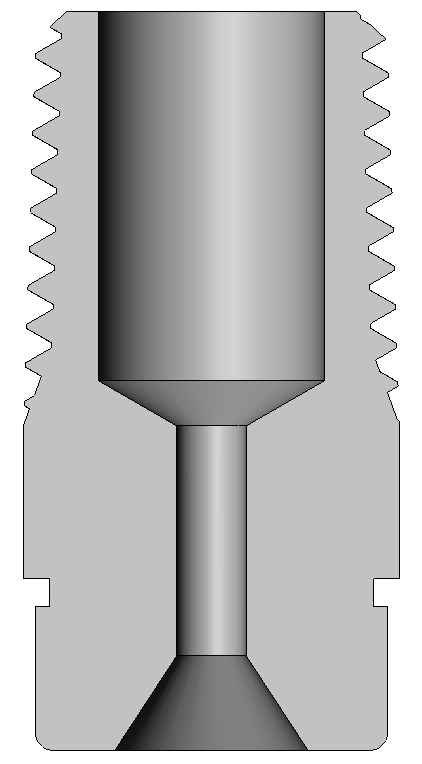
\includegraphics[height=0.3\textheight]{images/spray_nozzle.png}
        \end{figure}
    \end{minipage}
\end{frame}

\begin{frame}{McMaster-Carr nozzle}
    Instead of calculating, the flowrate and pressure drop could be supplied by the spray nozzle manufacture. In this case, we chose Mcmaster-Carr 32885K571 spray nozzle (\url{https://www.mcmaster.com/32885K571/}) 
    \begin{itemize}
        \item This spray nozzle is stainless steel
        \item This spray nozzle is $120^{\circ}$, full-cone type
        \item Flow rate at 100psi pressure drop is 4.6gpm
    \end{itemize}
\end{frame}

%=======================================================================================
\section{Design result}
\begin{frame}{Overall CAD file}
    \centering 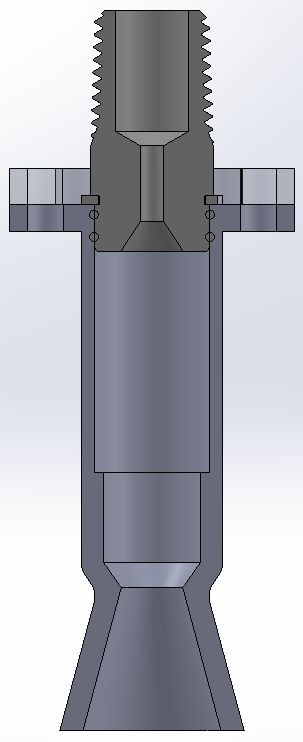
\includegraphics[height=0.9\textheight]{images/engine_assembly.png}
\end{frame}


%=======================================================================================

\section*{End-of-File}
{
\usebackgroundtemplate{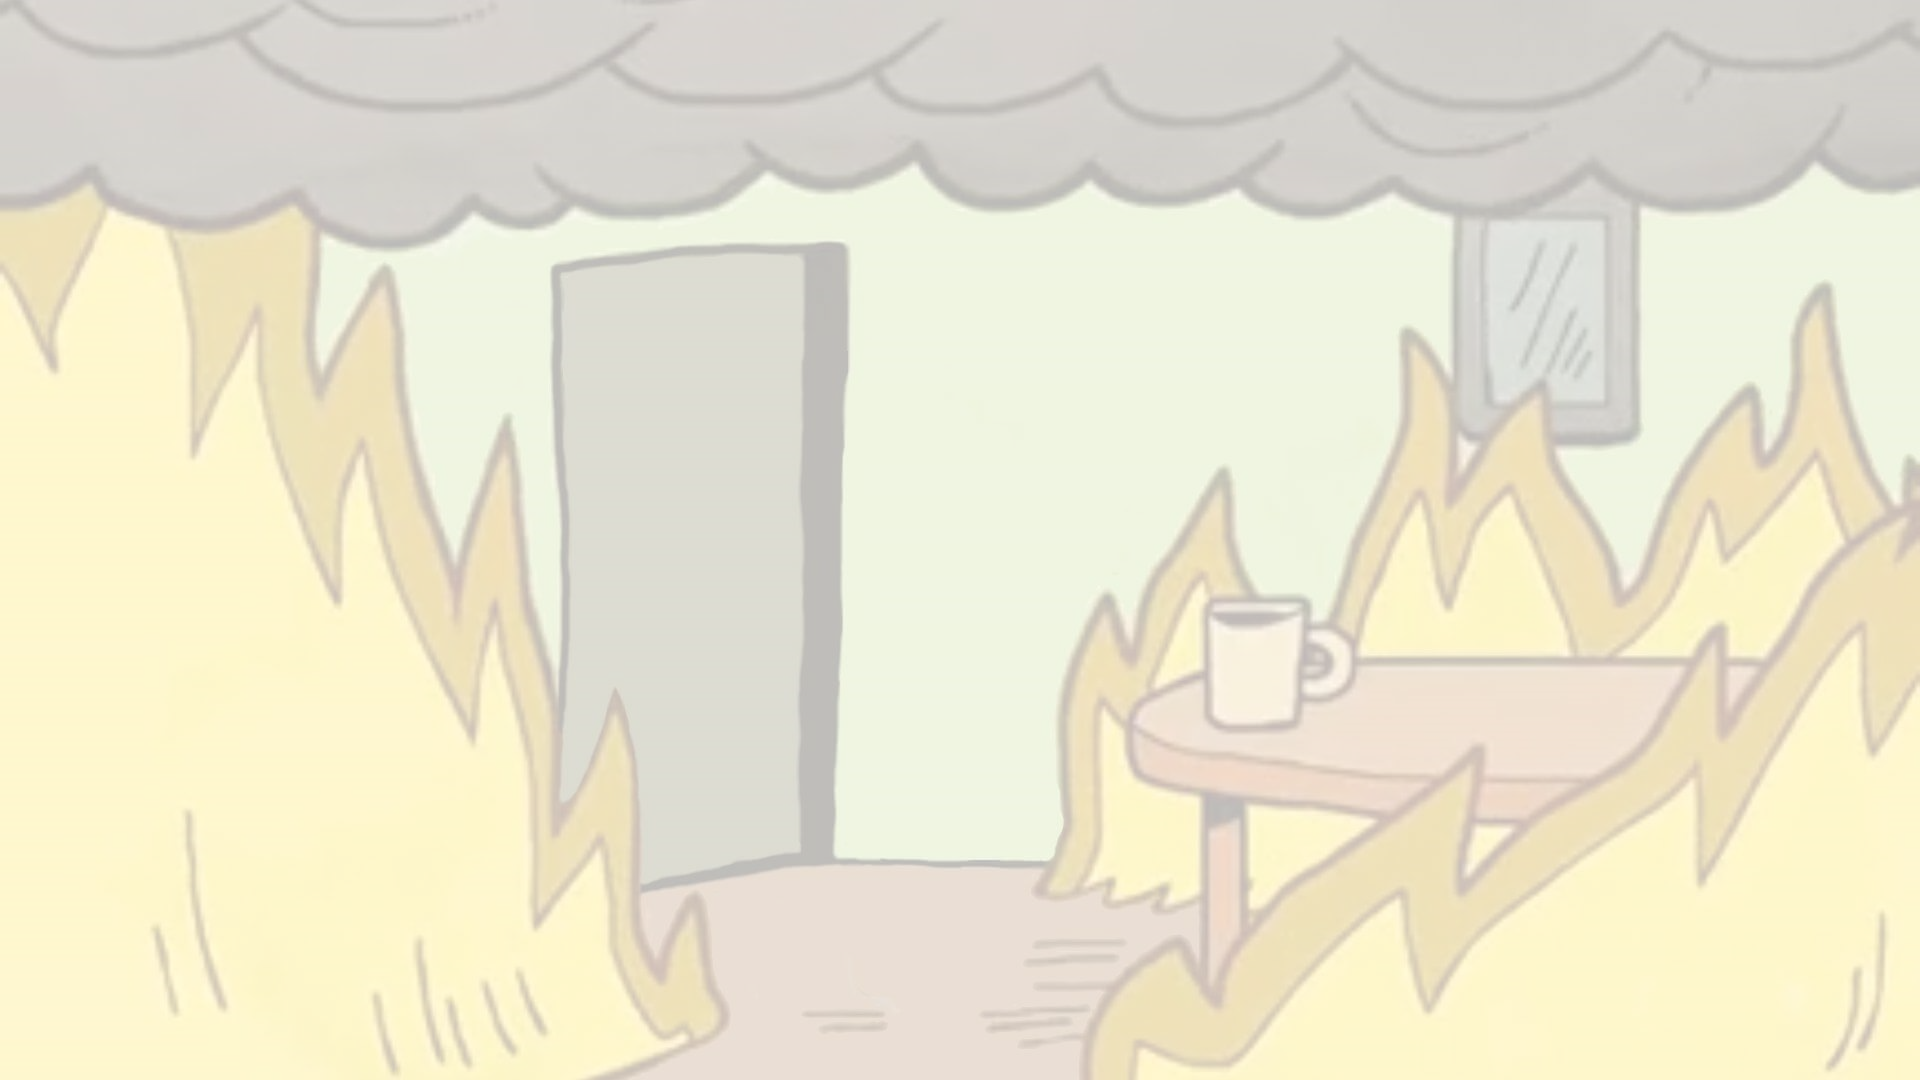
\includegraphics[width=18cm]{images/bg.png}}% make sure to reduce the opacity of the BG before uploading it
\begin{frame} 
    \maketitle
\end{frame}
}
\end{document}
